
\section{Chapter 3:\\ Can inverse calibration help improving process-based species distribution models?}
\label{chapter3}

\vspace*{1cm}
\sffamily
\large
\begin{center}
Victor Van der Meersch$^1$, Isabelle Chuine$^1$

\vspace*{0.1cm}
\small
\emph{$^1$CEFE, Univ Montpellier, CNRS, EPHE, IRD, Montpellier, France}
\end{center}

\vspace*{0.7cm}
\normalsize
%\textbf{Published in Methods in Ecology and Evolution:} \url{https://doi.org/10.1111/2041-210X.14119}

\vspace*{1.5cm}

\textbf{ABSTRACT}\\
Process-explicit models (PEMs) are expected to provide more reliable projections of species range shifts because they explicitly model biological mechanisms that govern species response to climate.
However, this kind of approach requires detailed and diverse data, which are available only for few species. 
Inverse calibration has been identified as an avenue to help calibrating PEMs for many species. However, it is still unclear whether it can yield correctly specified parameters.
Here, we explored the potential of such inverse calibration techniques to enhance the accuracy of PEMs. We calibrated a PEM (which focus on phenology) using species distribution data, following two strategies: (i) calibrating all parameters simultaneously or (ii) focusing only on critical parameters. We then evaluated the realism of the processes by comparing the simulations to phenological observations across Europe. 
We showed that model structure alone do not sufficiently constrain the calibration process, which may produce unrealistic parameter values. However, using inverse calibration parsimoniously can improve model performance while still allowing to simulate realistic processes.


\rmfamily

\newpage

\subsection{Introdution}

There have been repeated calls for focusing efforts on the development of process-explicit models in ecology \citep{Urban2016, Singer2016, Pilowsky2022}. Because they describe cause-to-effect relationships, they are assumed to provide more robust projections in novel climatic conditions. However, process-explicit models are still applicable to too few species \citep{Evans2016}, and their widespread use requires to address and to quantify their error and uncertainty.

We can distinguish two main source of errors in ecological models: the model's structure and the value of the parameters. The structure of a model is defined by its underlying assumptions and level of simplification. Our understanding of the regulation of the ecophysiological processes at the scale of organisms, that ultimately drive  ecosystem dynamics has grown substantially in the last decades. This has led to significant improvements in how we represent these processes in models, e.g. plant hydraulics \citep{Ruffault2022} , although some remains challenging, e.g. bud dormancy \citep{Chuine2016} or carbon allocation. 
These advancements enable researchers to explore complex interacting mechanisms, providing useful insights and tools for determining conservation and management strategies in a changing world \citep{Urban2016}. However, the incorporation of new detailed processes can become a trap \citep{Franklin2020}, as it often increases the number of poorly known parameters and limits the number of species for which these models can be applied. %parameter burden!

Indeed, process-explicit modeling depends a great deal on the calibration and the availability of data \citep{Cabral2017}. In a classical framework, parameters are typically determined from experiments, measurements, and expert knowledge. When it is too difficult or impossible, a cost-effective solution to the problem of estimating many parameters is the use of inverse modeling to bridge observations and simulations \citep{Evans2016}. This involves adjusting the parameters until the model outputs closely match the observed data, often using an optimization algorithm. Resulting parameter values are conditional on model structure and on observed data: the model structure explicitly constrains how climatic factors influence species performance, and the parameters and simulation outputs depend on the observations in a similar way to statistical models \citep{Zhang2024}. Inverse modeling is frequently used in process-explicit models to infer model parameters or at least some of them. Process-related data can be used to fit some part of the models separately or sequentially, e.g. tree ring series have been used to calibrate a sapwood growth submodel \citep{DeCaceres2023}, and phenological records are frequently used to calibrate phenological submodels \citep{Chuine2013}. Several data sources can also be combined to refine models \citep{BenitoGarzon2019} and to calibrate several processes simultaneously in a model-data fusion fashion \citep[e.g.][]{Trotsiuk2020}. This allows to integrate data at multiple spatiotemporal scales \citep{Hartig2012, Niu2014}, and reduce potential overfitting issues \citep{Bacour2023}.

However, being able to reproduce observed data, even from several sources, does not guarantee converging towards biologically sound parameter estimates. First, models are a simplification of reality for several reasons. Whether intentional or not, this simplification may miss important processes \citep{Forrester2021}, and inverse calibration may thus lead to parameter values that compensate for these missing processes. Second, even in a structurally correct model, measurements are not likely to coincide precisely with what the model simulates \citep{Zhang2024}. Third, some parameters might also be model-specific (i.e. conceptual?), and not correspond to something observable nor measurable.

Regarding process-explicit species distribution models, inverse modelling can benefit from species distribution data available across large scales \citep{Evans2016}. Traditionally, these data have only been used by correlative niche models, and attempts to use them to calibrate process-explicit models have been rare \citep{Higgins2012, VanderMeersch2023}, probably because this does not align well with the general idea of this modelling approach. While using only species occurrence data to infer the values of many parameters can be seen as a brute-force approach, such inverse calibrated process-explicit models may outperform correlative models and better reproduce the distributional patterns of the species on different spatio-temporal situations (\citealp{Higgins2020, VanderMeersch2024}; \hyperref[chapter2]{Chapter 2}).  Moreover, such inverse calibration could also help making them easier to apply to a greater number of species and on a larger scale \citep[e.g.][]{Conradi2024}. However, a good model fit to observations, even over a long-term period, does not necessarily imply a good estimation of the processes truly responsible for the observations. 
To reach high levels of confidence in model projections,  \cite{VanderMeersch2024} showed that ecological processes should still be simulated with a high level of mechanistic realism and that using species occurrence data alone to calibrate models may not provide the highest model performance, especially in novel conditions. 

Here, we investigate the differences between parameter estimates of a process-explicit model obtained either with a classical calibration or with inverse calibration, and what it implies in terms of realism of the simulated processes and of model performance. More precisely, we seek to understand whether and to what extent inverse calibration using species occurrence (i) can lead to realistic parameter values and processes and (ii) may help us improving process-explicit models. To do this, we focus on PHENOFIT, a process-explicit model which has been used to study species range determinants and to forecast species distribution shifts with past and future climate change in North America and Europe
\citep{Morin2007, Saltre2013, Saltre2015, Cheaib2012}. We first examine in detail 100 calibrations obtained for European beech (\emph{Fagus sylvatica} L.), and analyze the compensations between parameters and the realism of the simulated processes against observations all over Europe. We then investigate whether inverse calibration could improve parameter value estimation of some processes for which data are lacking for seven European forest tree species. 

\subsection{Materials and Methods}

\subsubsection{Process-explicit modeling with PHENOFIT}

PHENOFIT is a process-explicit model developed for temperate tree species which has been used to project their distributions using climatic conditions. It estimates the probability of presence of an adult tree defined as the product of the probability of survival and the probability of reproductive success at a yearly time step (i.e. fitness). 
Each phenological event (leaf unfolding, flowering, fruit maturation and leaf senescence) is simulated with daily climate forcing, and the model assumes that a tree species range depends mainly on the synchronization of its timing of development to the local abiotic conditions. Thus, for example, the fitness can be reduced when a severe drought event occurs between budburst and leaf senescence, or when a substantial proportions of leaves and flowers that take part to the development of the fruits are killed by frost. In the following, we will provide a more detailed description of three important processes of PHENOFIT, which will be discussed further in this article. A precise description of the submodels and the response functions can also be found in \hyperref[app:chapter3]{Appendix} for beech.

\paragraph{Leaf unfolding and flowering submodels}
Dates of leaf unfolding (date at which 50\% of leaves are unfold) and flowering (date at which 50\% of flowers are mature) are calculated using mechanistic phenology models \citep{Chuine2017}. Organ development is represented by a state variable, $S$ for development state, which is the integration of development rates ($R$) over time (in daily steps) from a start date $t_0$. The general structure of mechanistic phenology models for one specific development phase is the following:
$t_n$ such that $S_{n,t}$ = $\sum_{t=t_{n-1}}^{t_n} R_{n,t}$ = $S_n^*$ 
where $n$ is a development phase, $S_{n,t}$ is the state of development on day $t$ in phase $n$, $t_n$ is the end of phase $n$ and  $t_{n-1}$ the end of phase ${n-1}$, $R_{n,t}$ is the rate of development during phase $n$ on day $t$ which is a function of  temperature, and $S_n^*$ is the critical state required to reach $t_n$.  Several phases of developement can be modeled in a single model composed of several submodels each one describing a specific phase such as dormancy induction, endodormancy, ecodormancy, etc. In such case, phases either follow each other sequentially or can overlap depending on the development phase and the species. Leaf unfolding and flowering dates have been modelled here using 2-phases models describing both the bud endodormancy phase (bud remain dormant despite meteorological conditions that could sustain cell growth) and the ecodormancy phase (bud cell growth depends on the meteorological conditions).  Development rates ($R$) are response functions to daily temperature that can be linear or nonlinear (usually with a single optimum), and vary with the species and the development phase. 

\paragraph{Frost hardiness submodel}

Frost hardiness of vegetative and reproductive organs is modelled according to \citet{Leinonen1996}, as a function of the additive effect of photoperiod and temperature, and depends on the state of development (or phenological state): hardiness varies dynamically between a maximum value reached during bud winter dormancy and a minimum value reached at bud break and flowering. The model has several parameters, including the minimum level of frost hardiness $FH_{min}$ and the maximum level of frost hardiness ($FH_{max}$) conveyed both by photoperiod and temperature (see \hyperref[app:chapter3]{Appendix} for a detailed description of the model). 

\paragraph{Fruit maturation submodel}

Fruits development is modeled with a two-phases mechanistic phenology model:  a first phase of cell multiplication and growth, and a second phase of photosynthetic assimilate accumulation. This second phase is the most important, and depends on several components including the proportion of leaves that resisted frost, water availability and photosynthetic activity. The latter varies according to temperature conditions following the unimodal function of \citet{Wang1998} which involves an optimal temperature parameter $T_{opt}$.  Fruit maturation is integrated over time at the scale of the tree crown, following a normal distribution. The mean date of fruit maturation corresponds to the date when fruit development reaches $Mat_{moy}$, and correspond to the stage 50\% of fruits are ripe,  and fruit maturation starts at $Mat_{moy}$ $-3\sigma$ and ends at $Mat_{moy}$ $+3\sigma$.

\paragraph{Leaf senescence submodel}
Leaf senescence date (date at which 50\% of leaves have changed color) is modelled using a 1-phase mechanistic phenology model with different response functions to temperature and to day length depending on the species \citep{Delpierre2009}. 

\paragraph{Climate and soil data used to run the model}

Historical simulations (1970-2000) were run with climate variables extracted from the ERA5-Land hourly dataset \citep{MunozSabater2021}. As in \citet{VanderMeersch2023}, we computed daily mean values of several variables: temperatures (minimum, mean and maximum), dewpoint temperature, precipitation, global radiation and wind speed. Daily potential evapotranspiration was calculated using the standard FAO Penman–Monteith equation \citep{Allen1998}. Soil water holding capacity was calculated with the field capacity and wilting point data from EU-SoilHydroGrids \citep{Toth2017} and the percentage of coarse fragments from SoilGrids250m \citep{Hengl2017}.

Paleosimulations were run using the same climatic forcing as in \citet{VanderMeersch2024}. Daily data were generated, using the weather generator GWGEN \citep{Sommer2017}, from the monthly simulations of HadCM3B-M2.1 coupled general circulation model \citep{Armstrong2019}.

\subsubsection{Model calibration}

\paragraph{Expert calibration}

PHENOFIT has been calibrated for several European tree species, and validated  by comparing their historical and Holocene distribution to the modelled fitness  \citep{Saltre2013, Duputie2015, Gauzere2020, VanderMeersch2024}. Some parameters were directly measured or found in the literature, e.g. the frost hardiness submodel parameters. Phenology submodel parameters were inferred by inverse modelling using phenological data across Europe (provided through the 
\href{https://data.pheno.fr}{TEMPO} data portal, and the \href{https://pep725.eu}{PEP725} database). %Finally, a few parameters are prescribed based on expert knowledge as no data to estimate them exist. 
This expert calibration of the model does not involve species occurrence data at any point.

\paragraph{Inverse calibration with CMA-ES algorithm and species occurrence data}

Following \citet{VanderMeersch2023}, we calibrated PHENOFIT using the covariance matrix adaptation evolution strategy (CMA-ES), which  is a robust algorithm for complex optimization problems \citep{Hansen2001}. It is inspired by Darwin's theory of evolution to find the most fit parameter sets. We ran the CMA-ES calibration on the multicore cluster GenOuest (\url{https://genouest.org}).

The objective function for the calibration was the area under the receiver operating characteristic curve (AUC), to maximize model discriminating capacity (i.e. potential to distinguish between species presences and absences). To compute the AUC, we used the same occurrence data as in \citep{VanderMeersch2023}. These were mainly extracted from the EU-Forest dataset \citep{Mauri2017}, completed with presence records extracted from the Global Biodiversity Information Facility (\url{https://gbif.org}) to account for tree occurrences outside forests. We removed GBIF occurrences outside natural species ranges as defined by Atlas Flora Europeae \citep{AFE2005} and EuroVegMap \citep{EVM2003}. In order to reduce calibration computational costs, we selected subsets of 1000 occurrences,  based on a k-means clustering to make sure that all species environmental preferences were proportionally represented (see \citet{VanderMeersch2023} for details). The EU-Forest cells where the species is not reported present were considered as (pseudo-)absences.

First, we ran one hundred calibrations for \emph{Fagus sylvatica}, using species occurrences and the same parameter bounds as in \citet{VanderMeersch2023} in order to remain in realistic parameter ranges. These calibrations are called \emph{full} inverse calibrations in the following (all parameters optimized at once). Second, we ran a second set of inverse calibrations, for seven different species (\emph{Abies alba}, \emph{Betula pendula}, \emph{Fagus sylvatica}, \emph{Larix decidua}, \emph{Picea abies}, \emph{Quercus pubescens} and \emph{Quercus robur}), to optimize only a subset of parameters. These parameters corresponded to processes that we identified as responsible for false absence errors (\Cref{fig:4}) in the predictions of the expert calibration version of the model. Other parameters were fixed at the expert values. For each species, we ran 5 calibrations on 2 different occurrence subsets (i.e. 10 repetitions). These calibrations are called \emph{partial} inverse calibrations in the following. 

\subsubsection{Parameter estimates' evaluation}

We partitioned the 100 \emph{full} inverse calibrations of \emph{Fagus sylvatica} using two k-means clustering procedures in a row (\Cref{fig:2}). The first clustering was based on the simulated leaf dormancy break and leafout dates. Then, within each cluster, the second clustering was computed based on the fruit maturation and leaf senescence dates.

In order to verify that the parameter values after calibration lead to realistic processes, we calculated root-mean-square errors between simulated phenological dates and observed dates. The latter were extracted from two databases, PEP725 and TEMPO, covering the period 1970-2000, essentially in Central Europe (\Cref{fig:phenologicalrecords}). For Fagus sylvatica, we used N observations of leafout, N of flowering, N of fruit maturation and N of leaf senescence (\Cref{fig:3}). Moreover, we used N obs. of Betula pendula flowering, N obs. of Picea abies flowering and N. obs of Quercus robur fruit maturation (\Cref{fig:5}).

% Clustering des calibrations...\\
% Main limiting factors (fig4)...\\

\subsection{Results}

\subsubsection{Coherent and stable predictions despite process discrepancies}

The similarity between the simulated ranges of European beech obtained with the 100 \emph{full} inverse calibrations was relatively stable over the last 12k years. The disagreements were mostly at the margins of the distribution (\Cref{fig:1B,,fig:1D}). The S\o rensen dissimilarity between the inverse calibration projections was lower in historical conditions (median = 0.0805 [IQR = 0.0605 - 0.106]) than in the distant past, e.g. 11,500 years ago (0.116 [0.0813 - 0.154], \Cref{fig:1E}). However it increased relatively little compared to the dissimilarity with the expert calibration, from 0.276 [0.268 - 0.283] in the present to 0.410 [0.391 - 0.429] at 11,500BP.

These relatively similar projections, however, resulted from different intermediate processes (\Cref{fig:2}). Regarding bud development, 65 calibrations (clusters blue and green, \Cref{fig:2A})  had a short endodormancy phase (ending in November or December of the previous year, \Cref{fig:2B}) and a longer ecodormancy phase (with an average duration of 187 days $\pm$ 56.9). On the contrary, the remainder of the 34 calibrations (clusters yellow and orange, \Cref{fig:2A}) had a longer endodormancy phase (ending in February or March) and a shorter ecodormancy phase (with an average duration of 89.4 days $\pm$ 38.7). Note that one of the calibrations stood out due to both short endodormancy and short ecodormancy (\Cref{fig:2B,,fig:2C}). Similarly, two behaviors can be identified in terms of fruit maturation: 83 calibrations (clusters green and yellow) led to early maturation (August/September, \Cref{fig:2D}), and 16 led to late maturation (October/November, \Cref{fig:2D}).


\begin{figure}[htpb]
\centering
\begin{subcaptiongroup}
\phantomcaption\label{fig:1A} 
\phantomcaption\label{fig:1B}
\phantomcaption\label{fig:1C}
\phantomcaption\label{fig:1D}
\phantomcaption\label{fig:1E}
\end{subcaptiongroup}
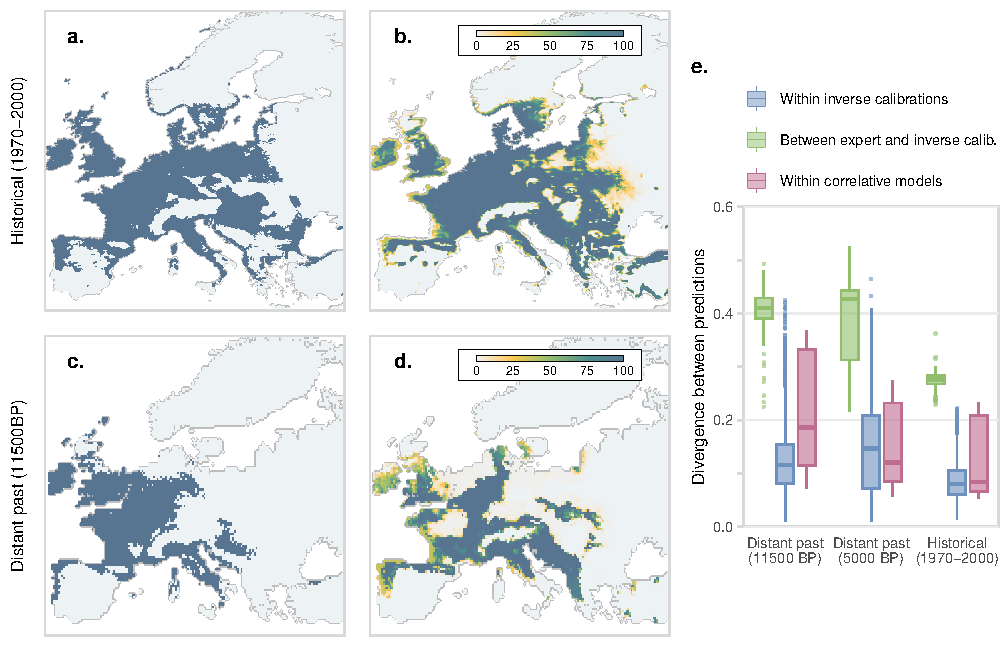
\includegraphics{chapter3/figs/fig1-1.pdf}
\caption{Simulated presence of \emph{F. sylvatica} with \textbf{(a,c)} the expert parametrization and \textbf{(b,d)} the set of 100 \emph{full} inverse calibrations, in the historical climatic conditions \textbf{(a,b)} and in the paleoclimatic conditions \textbf{(c,d)}. \textbf{(e)} S\o rensen dissimilarity between inverse calibrations, and between expert calibration and inverse calibrations. S\o rensen dissimilarity between 5 different correlative models is shown for comparison. BP stand for "Before Present" (1950).}
\label{fig:1}
\end{figure}

\begin{figure}[htpb]
\centering
\begin{subcaptiongroup}
\phantomcaption\label{fig:2A} 
\phantomcaption\label{fig:2B}
\phantomcaption\label{fig:2C}
\phantomcaption\label{fig:2D}
\phantomcaption\label{fig:2E}
\end{subcaptiongroup}
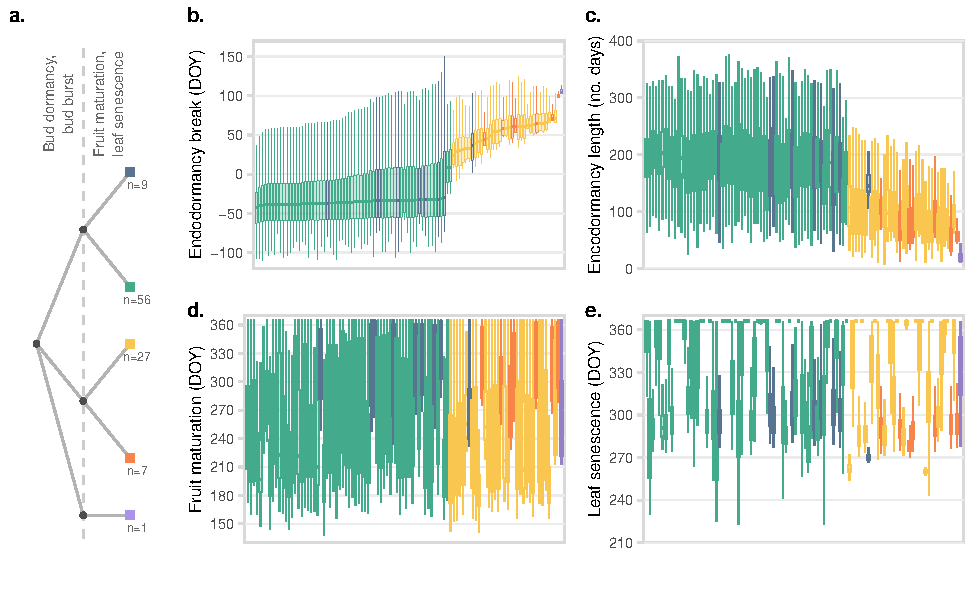
\includegraphics{chapter3/figs/fig2-1.pdf}
\caption{\textbf{(a)} Partition of the 100 inverse calibrations for \emph{F.sylvatica} after a two-step clustering based on the phenological processes simulated: \textbf{(b)} bud endodormancy, \textbf{(c)} bud ecodormancy, \textbf{(d)} fruit maturation and \textbf{(e)} leaf senescence. Note that we do not show flowering as it occurs almost simultaneously with budburst, since beech buds are mixed.}
\label{fig:2}
\end{figure}

\subsubsection{Errors in the simulated processes}

These strong discrepancies between simulated processes inevitably led to differences in terms of agreement with phenological observations across Europe (\Cref{fig:3}). The first group of calibrations (short endodormancy/long ecodormancy) had a median error of 28.3 days for the budburst date, and up to 120 days for the worst calibration. The second group (long endodormancy/short ecodormancy) had a smaller median error of 16.3 days [7.73 - 27.4]. Both performed worse than the expert version of the model (6.95 days [3.36 - 12.1], \Cref{fig:3A}) whose parameters were calibrated using some of these observations. Regarding fruit maturation, the late-maturation cluster (blue and orange) got a median error of 17 days [8 - 29], closer to the expert version (13 days [6 - 24]). Moreover, inverse calibrations showed almost no year where fruit maturation could not occur while it was observed, unlike the expert version, whose parameters did not allow for ripe fruits in more than 50\% of the cases (\Cref{fig:3C}). On the contrary, for senescence, 43\% of the calibrations led to no senescence date for at least 50\% of the cases (\Cref{fig:3D}), and 34\% to no senescence at all. These calibrations belonged exclusively to the early-maturation cluster (green and yellow), whereas the late-maturation cluster got a median error of senescence date of 14.6 days [8.75 - 22], slightly higher than the expert version (10.8 days [6 - 16]).

\begin{figure}[htpb]
\hspace*{-1cm}
\centering
\begin{subcaptiongroup}
\phantomcaption\label{fig:3A} 
\phantomcaption\label{fig:3B}
\phantomcaption\label{fig:3C}
\phantomcaption\label{fig:3D}
\phantomcaption\label{fig:3E}
\end{subcaptiongroup}
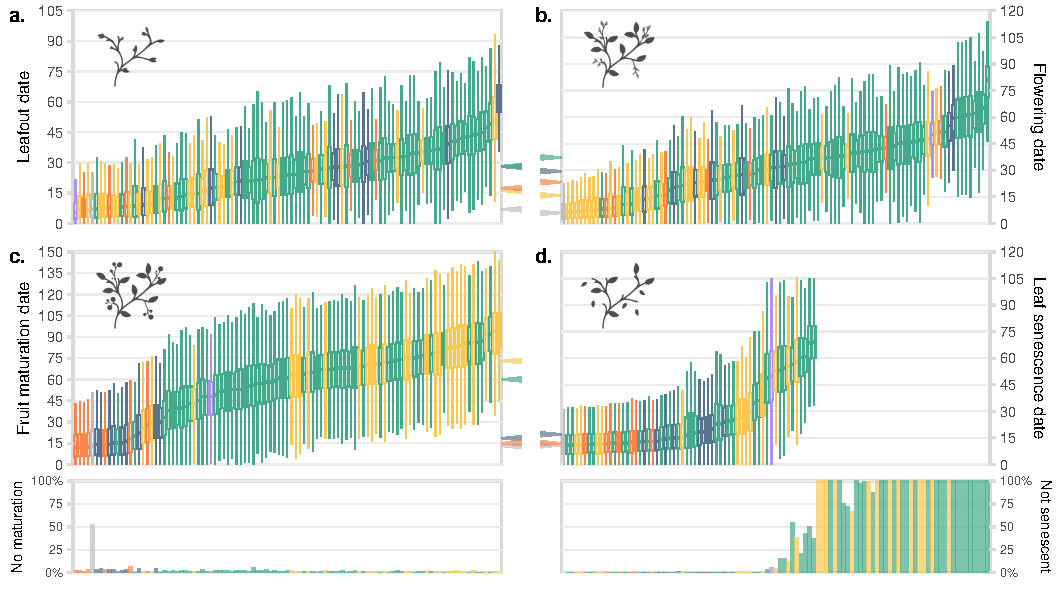
\includegraphics{chapter3/figs/fig4-1.pdf}
\caption{Root-mean-square error (RMSE) between phenological dates that were observed (between 1970 and 2000) and those that were predicted by the different calibrations, for \textbf{(a)} leaf unfolding, \textbf{(b)} flowering, \textbf{(c)} fruit maturation and \textbf{(d)} leaf senescence. For fruit maturation and leaf senescence, the lower panels show the percentage of observations for which the parameter sets predicts that the event does not occur (i.e. no maturation or no leaf senenescence). Colors are based on the clustering shown in Fig. 2, grey corresponds to the expert parameter set. Arrows in the middle indicate the median RMSE for each group.}
\label{fig:3}
\end{figure}

\subsubsection{Partial calibrations on selected parameters}

The previous results showed significant differences between the calibrations in terms of simulated processes and of agreements with the available observations. However, some of the calibrations simulated processes that were relatively consistent with observations, and this was confirmed in the following when attempting to inversely calibrate the processes causing false absence errors with the expert version of the model. Most partial calibrations resulted in an AUC higher than 0.8 (\Cref{fig:4}), and in the best-case scenario an increase of more than 0.4 for spruce \emph{(Picea abies}), where we transitioned from a model worst than random to one with a good discriminatory ability.

The lack of data, particularly for fruit maturation, prevented us from checking the realism of partial calibrations for all species. We were able to evaluate the inverse calibrations of the fruit maturation date submodel for beech (\emph{Fagus sylvatica}) and pedunculate oak (\emph{Quercus robur}, \Cref{fig:5A}), of the flowering date submodels for birch (\emph{Betula pendula}) and spruce  (\emph{Picea abies}, \Cref{fig:5B}), and the frost hardiness submodel for fir (\emph{Abies alba}), beech and birch (\Cref{fig:5C}). For beech, most calibrated parameter sets converged towards a median error of the fruit maturation date ranging from 11 to 16 days (except one with a median error of 24 days), close to the expert version error of 13 days (\Cref{fig:5A}). Similarly to the full calibrations, they also corrected the non-fruit maturation issue of the expert version. For pedunculate oak , half of the calibrations led to errors in the fruit maturation date similar to the expert version, around 16 days, and only 9.67 days [4.33 - 17] for the best parameter set (\Cref{fig:5A}). Regarding the flowering date of birch, 2 out of 10 partial calibrations resulted in a lower median error (5.91 days [2.55 - 11.6] and 5.91 days [2.72 - 11.4]) than the expert parameter set (8.87 days [4.21 - 14.9]). However, some had a much higher median error, up to 50.2 days (\Cref{fig:5B}). For spruce, the best calibration in terms of RMSE simulated no flowering in 37.3\% of the cases. Apart from this one, the other 9 calibrations had a higher median error (between 18.3 days [10.3 - 27.9] and 29.7 days [20.0 - 41.7]) than the expert version of the model (11.5 [5.68 - 18.9]). Finally, the frost resistance submodel parameters were very close to the expert version in only one third of the cases (\Cref{fig:5C}).

\begin{figure}[htpb]
\hspace*{-0.5cm}
\centering
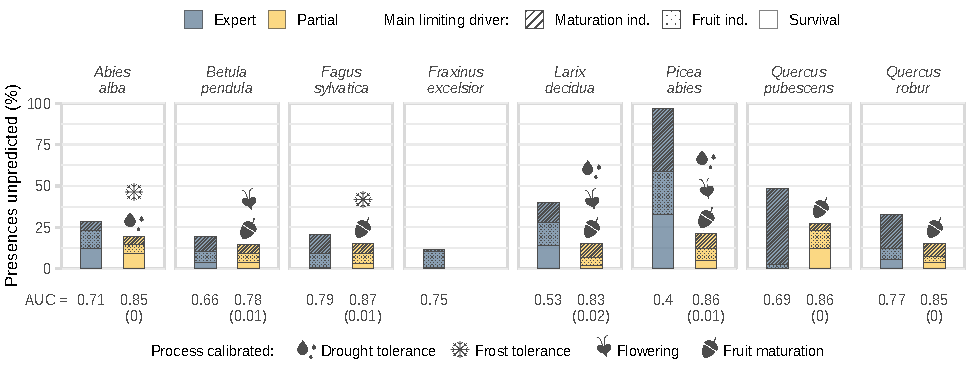
\includegraphics[width=30cm]{chapter3/figs/fig6-1 - icons.pdf}
\caption{Results of the \emph{partial} calibrations for the seven species considered, where only some of the parameters were optimized. The y-axis shows the percentage of observed presences that are predicted as absences by the model (i.e. \emph{false absences}), and the bar patterns represent the main simulated processes explaining these errors. The bottom row shows the average AUC (a classic discrimination performance metric) and its standard deviation in parenthesis.}
\label{fig:4}
\end{figure}

\clearpage

\subsection{Discussion}

Our results show that inverse calibration of process-explicit models using species distribution data does not necessarily lead to realistic parameters and simulated processes. They further demonstrate that inverse calibration can be highly useful as a model diagnostic tool, and, more importantly, to calibrate selected parts of a model where specific data and expert knowledge are lacking, albeit important cautions.

\begin{figure}[htpb]
\hspace*{-1cm}
\centering
\begin{subcaptiongroup}
\phantomcaption\label{fig:5A} 
\phantomcaption\label{fig:5B}
\phantomcaption\label{fig:5C}
\end{subcaptiongroup}
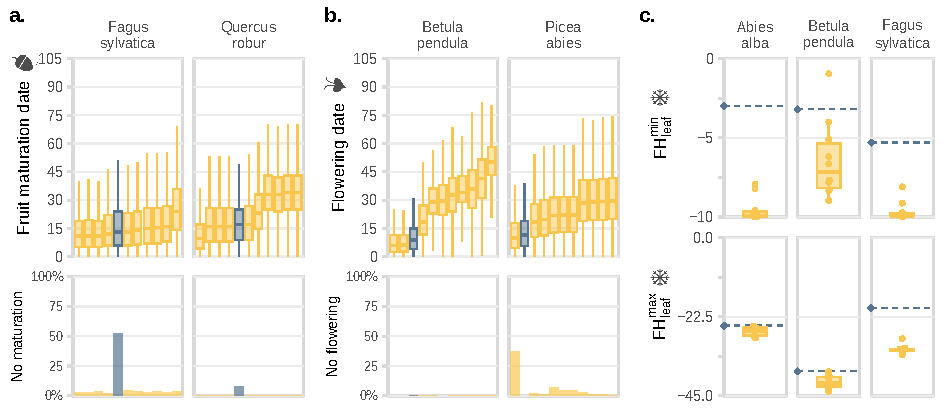
\includegraphics{chapter3/figs/fig7-1 - icons.pdf}
\caption{Root-mean-square error (RMSE) between phenological dates that were observed (between 1970 and 2000) and those that were predicted by the partial calibrations (yellow) and the expert calibration (blue), for \textbf{(a)} fruit maturation and \textbf{(b)} flowering. \textbf{(c)} represents the values of the frost hardiness parameters after partial calibration. The blue dotted line shows the expert value.}
\label{fig:5}
\end{figure}

\subsubsection{Inverse calibration can lead to accurate species range predictions despite unrealistic parameter estimates}

Some parameter sets outperformed the expert calibrations used for this study (especially when few data are available for the expert calibration), but most resulted in larger errors, up to 2 months in the worst case (\Cref{fig:3}). For some processes, inverse calibration induced even unrealistic functional traits. For example, a large portion of the calibrations considered beech as an evergreen species, or at least not senescent, in some areas (\Cref{fig:3D}).

Despite similar predictions of species distribution (\Cref{fig:1B}), we observed that simulated processes could strongly diverge between calibrated models. Some calibrated models led for example to a short endodormancy phase, followed by a longer ecodormancy phase, and \textit{vice-versa} (\Cref{fig:2A,,fig:2B}). This arises because the compensation between these two processes has little effect on the functional trait they regulate, the leaf unfolding date, and thus on the predicted distributions. The non-identifiability of parameter values obtained with inverse calibration is a known issue \citep{He2017, Cameron2022, VanderMeersch2023}, when different sets of parameters may result in equivalent model outputs. Here we show that compensations can occur between components of a same process or between different processes. For example, errors between simulated and observed leafout dates vary greatly across calibrated models (\Cref{fig:3A}), suggesting that these errors are compensated by another process for example leaf frost hardiness or fruit development. 

Unexpectedly, these discrepancies in the simulated individual processes did not cause a sharp increase in the dissimilarity between the predictions of the different calibrated models over the Holocene (\Cref{fig:1C,,fig:1D,,fig:1E}), even in the very different climatic conditions of the Early Holocene (\Cref{fig:dissimilarity}). In other words, while inverse calibrations led sometimes to very different parameter sets and thus very different "phenotypes" (early/late budburst, deciduous/evergreen...), the predictions nevertheless remained consistent across long time scales and novel climatic conditions. Therefore, the optimization algorithm manages to find consistently a similar relationship between climatic conditions and the higher-level model output (fitness), regardless of the divergent lower-level processes (frost hardiness, fruit development, etc). The link between climate and species distribution as captured in the occurrence data thus seems to constrain the model's behavior without necessarily capturing the realistic underlying processes. The strength of the optimization algorithm is also its weakness: it appears to accommodate the model structure, making it flexible enough to fit the data well. The model structure and the mathematical functions used to describe the processes are thus not sufficient to constrain the parameter estimates. Thus, contrarily to what is usually assumed \citep{Higgins2020}, here we find that process-explicit models are not necessarily less flexible than correlative models because of their structure. This highlights the importance of not focusing solely on some metrics of (apparent) performance, even in novel climatic conditions, but rather investigating the intermediate outputs of the model.

Finally, and similarly to correlative models \citep{BarbetMassin2010, Duputie2014},  process-explicit models are affected by the bias in the occurrence data used for the calibration. For example, all simulations predict a low beech fitness in south-west France contrary to the expert model predictions (\Cref{fig:1B}), whereas its absence is potentially more attributable to the legacy of forest management (vast maritime pine plantations) than to truly limiting climatic conditions as the presence of some old relict beech forests in the region suggests \citep{Lafontaine2014}.

\subsubsection{Inverse calibration can help identifying model limitations and opportunities for improvement}

Our results reveal both the power and the shortcomings of inverse calibration in ecological modelling, and call for a careful use of the method when one aims at providing projections in very different conditions from the calibration conditions. They further suggest that inverse calibration can be an effective diagnostic tool to improve  process-explicit models, both in terms of model hypotheses and parameterisation. Using species occurrence data to calibrate such models might be fruitful, if a detailed evaluation of the realism of the parameter estimates and the values of the functional traits (phenotypes) they produce is carried out.

Inverse calibration can help identify processes that are not accounted for, or incompletely accounted for in the model, even though they may be important in the context of the study, and reversely identify processes taken into account in the model which have little impacts on the targeted outputs. For example, the discrepancies between leaf senescence date predictions across the different calibrations (\Cref{fig:2D,,fig:3D}) highlight that, in the model, leaf senescence date is more weakly constrained by the calibration data compared to other traits because it has more limited impact on fitness. More precisely, late senescence dates have no impact on fitness because there is no nutrient remobilization in the model that would confer an advantage in loosing leaves before the first frost event, while early dates do when they occur before fruit maturation has finished. In this example inverse calibrations indicate that it might be opportune to refine the model by adding nutrient remobilization.

Using inverse calibration with species occurrence data can further improve process-explicit models in several ways. First, it can help improving the modelling of processes that have a significant impact on the model outputs but for which we have limited measurements and observations. For example, for forest tree species, observations of fruit maturation are often sparse and limited to some areas. It is therefore difficult to find the correct parameter values for the fruit maturation submodel, which can cause errors (e.g. frequent lack of maturation for beech, \Cref{fig:3C}). Relaxing the fruit maturation submodel parameters in the expert version of the model for several species and calibrating them using inverse calibration and species occurrence data (\Cref{fig:4}) not only increased the goodness-of-fit of the models as expected, but also resulted in more accurate predicted fruit maturation dates on average (\Cref{fig:5A}).
Second, as pointed by \cite{Harrison2021}, the estimation of process-explicit model parameters are sometimes \emph{ad hoc} or rely on outdated data. Thus \emph{partial} inverse calibration can also be an opportunity to identify the parameters where the disagreement between the expert value and the calibrated values is systematically significant, which could indicate the need to reassess the expert values. For example, the maximum frost resistance of buds during winter, ${FH}^{max}$ , used in the expert version of the model for \emph{beech} is higher (-20°C; \citealt{Till1956, Lenz2013})  than the value obtained by inverse calibration (-32°C on average, \Cref{fig:5C}) which is closer to more recent studies \citep{Delaporte2015, Hofmann2015, Kreyling2014, Lenz2016}. 
 
However, we should keep in mind that the parameter values inferred with such \emph{partial} calibrations are conditioned by the rest of the fixed processes and by the structural errors and hypotheses of the model. For example, the minimum frost resistance of leaves at leaf unfolding, ${FH}^{min}$, converged towards an unrealistically low value of -10°C for both beech and fir (the lower bound constraining the optimization of this parameter; \Cref{fig:5C}). This may have at least two explanations. First, the parameters of the leaf unfolding submodel might actually be not valid for the entire study area (e.g. existence of local adaptation of populations to climatic conditions; \citealp{Kreyling2014}) and the calibration algorithm compensated too early leaf unfolding date with a higher frost resistance of leaves. Second, the model does not account for possible different resistance to frost between a freshly unfold leaf and a mature leaf, which may have biased the estimation of ${FH}^{min}$.  

\clearpage

\subsubsection{Inverse calibration can provide a more comprehensive assessment of model uncertainties}

In many process-explicit model applications, parameter uncertainties are not considered and simulations are run with a single parameter sets \citep{Niu2014, Lobell2010}. Typically, in previous studies using PHENOFIT, all parameters had a chosen fixed value, and model deterministic outputs did not account for parameter uncertainties. To avoid being overconfident with individual model projections, multiple inverse calibrations could be used to generate an ensemble of model projections (\Cref{fig:1B}). The spread of model outputs across the ensemble may then allow to assess the uncertainty associated with the parameter values \citep{Simmonds2024}, and to provide a more comprehensive range of projections rather than single deterministic outcomes.

However, these projections will always be contingent on model hypotheses and structure. The representation of processes in models may indeed represent a large source of uncertainty, as processes can usually be modeled with various equations determining their functional form \citep{Keenan2011b}. One could test a set of alternative mathematical structure to quantify the impacts of this structural uncertainty \citep{Huber2020}. An efficient way could be to include them during the calibration procedure, i.e. by also optimizing similarly plausible process formulations rather than just the parameter values.

Overall, inverse calibration using species distribution data show promise as a method to enhance specific model components in the absence of more precise data. However, process-explicit model structure and mathematical functions alone do not sufficiently constrain the calibration process. To avoid producing unrealistic parameter estimates, inverse calibration thus necessitates a careful application and a thorough evaluation to ensure realistic modeling outcomes. In the near future, the increasing availability of high-resolution data -- such as remote sensing or LiDAR, combined with an effective inverse-calibration framework, will enable a continuous integration of large-scale data and ultimately a better model parameterization.